\subsection{Reservoir transfer-supply model with possible external water transfer}
The simulation and optimization method is used to study the operation and scheduling of reservoirs with possible external water transfers, which is divided into two parts: the simulation module and the optimization module. The simulation module is based on water distribution, water transfer and water supply rules to adjust and calculate external water transfer and natural water supply, and set water transfer and water supply rules for the inflow reservoirs to meet the remaining demand as much as possible; the optimization module is based on the analysis of reservoir scheduling performance to optimize the set water transfer and water supply rules.
% TO DO
\begin{figure}[H]
 \centering
 \label{figure2}
 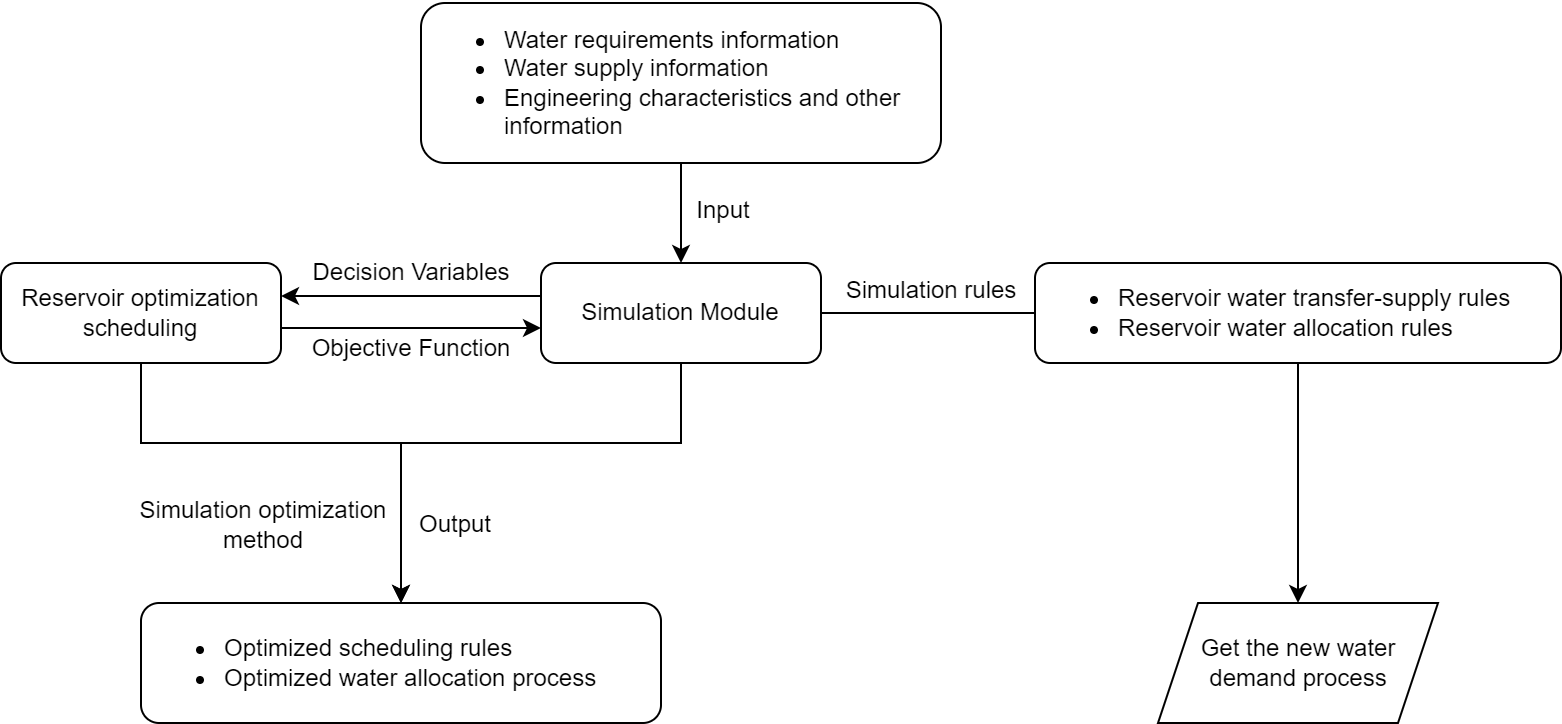
\includegraphics[width=0.8\textwidth]{figures/allc.png}
 \caption{Model Framework Diagram}
\end{figure}
\subsubsection{Analog Module}
\begin{enumerate}[(1)]
 \item The existence of external water transfer when the deployment rules.The process of blending natural water and external water transfer is:
   \begin{itemize}
   \item Calculate the new storage volume for user i at time t: $ N_{t}^{i}=D_{t}^{i} $ , Where, $ D_{t}^{i} $ is the water demand of user i at time t.  This storage volume is deployed using the following reservoir transfer-supply rules.
   \end{itemize}
  \item Reservoir water transfer - water supply rules. According to the theory of reservoir capacity zoning, four scheduling lines are set up for the receiving side to control the transfer and supply of water from the reservoir. When the initial reservoir storage is above the start line $ S_{Y} $, the reservoir can supply water without external water transfer. Otherwise, water is transferred according to the reservoir's time transfer capacity $ Y^{max}_{t} $ and the maximum external transfer flow $ Z^{max}_{t} $. The other three scheduling lines $ S_{1} $, $ S_{2} $ and $ S_{3} $ restrict water supply to agricultural, industrial and residential users at a time, which are called water supply restriction lines. ~\cite{water_transfer_triggering_mechanism}
  %\begin{figure}
    %\centering
    %\includegraphics[width=0.8\width]{figures/analog_model.jpg}
  %\end{figure}
  \par
  In time t, the reservoir transfer-supply operation is as follows:
    \begin{itemize}
      \item When the initial storage volume $ V_{t} $ is above the start line $ S^{Y}_{t} $, the reservoir transfer volume $Y_{t}=0$. Otherwise, the water is transferred according to the transfer capacity $Y^{max}_{t}$ and the transfer flow $Z^{max}_t$.
      \item Determine the relationship between the initial storage volume $ V_{t}$ and the water supply limitation lines $S^{1}_{t}, S^{2}_{t}, S^{3}_{t}$ for each user at time t:
       \begin{enumerate}
          \item If $V_{t} \geq S^{1}_{t}$, each customer is supplied with water on demand:
            \begin{equation}
            W_{t}=N^{1}_{t}+N^{2}_{t}+N^{3}_{t}
            \end{equation}
          \item If $S^{2}_{t}\leq V_{t} \leq S^{1}_{t}$, water supply for agricultural users is restricted:
            \begin{equation}
              W_{t}=(1-\alpha_{1})\cdot N^{1}_{t}+N^{2}_{t}+N^{3}_{t}
            \end{equation}
          \item If $S^{3}_{t}\leq V_{t}\leq S^{2}_{t}$, water supply for agricultural users and industrial users is restricted:
            \begin{equation}
              W_t=(1-\alpha_1)\cdot N^1_t+(1-\alpha_2)\cdot N^2_t+N^3_t
            \end{equation}
          \item If $V_t\leq S^3_t$, water supply for all users is restricted:
            \begin{equation}
              W_t=(1-\alpha_1)\cdot N^1_t+(1-\alpha_2)\cdot N^2_t+(1-\alpha_3)\cdot N^3_t
            \end{equation}
       \end{enumerate}
      \item Calculate the water storage at the end of the period:
        \begin{equation}
          V_{t+1}=V_t+I_t+Y_t-W_t-q_t
        \end{equation}
        Where, $W_t$ is the total reservoir water supply at the time, $N^i_t$ is the water demand of agricultural, industrial and residential users at time t respectively; $\alpha^i$ is the water supply limitation coefficient of user i, $I_t$ is the incoming reservoir water at time t; $Y_t$ is the reservoir water transfer at time t, $q_t$ is the reservoir abandonment at time t.
    \end{itemize}
\end{enumerate}
\subsubsection{Optimization Module}
\paragraph{Objective Function}
When there is an external water source, it is not reasonable to abandon a large amount of water due to the limitation of reservoir capacity. In order to improve the efficiency of external water supply, we need to ensure that the amount of water abandoned by the reservoir is as small as possible, and set the objective function as:
\begin{enumerate}[(1)]
  \item Minimize the sum of squares of water deficiency
    \begin{equation}
      \min{f_1}=\sum^N_{t=1}\frac{N_t-W_t}{N_t}
    \end{equation}
    $N_t$ is the total water demand.
  \item Minimize annual average reservoir disposal
    \begin{equation}
      \min{f_2}=\frac{1}{T}\sum_{t=1}^N q_t
    \end{equation}
    Where, $T$ is the number of years, $q_t$ is the total amount of water abandoned by the reservoir, the smaller the amount of water abandoned, the higher the utilization rate of external water sources.
\end{enumerate}
\paragraph{Binding Conditions}
\begin{enumerate}[(1)]
  \item Balance reservoir initial and final water constraints
    \begin{equation}
      V_{t+1}=V_t+Y_t+I_t-W_t-q_t
    \end{equation}
    Where, $V_{t+1}$ and $V_{t}$ denote the initial and final water demand of the reservoir at time t respectively.
  \item Reservoir Capacity Constraints
  \par
  Due to the functional and mechanical characteristics of the reservoir, the water demand at each time must be within a certain range.
  \begin{equation}
    S^{min}_t\leq V_t\leq S^{max}_t
  \end{equation}
  Where, $S^{min}_t$ is the minimum storage limit,$S^{max}_t$ is the maximum storage limit.
  \item Water Demand Constraint
    \begin{equation}
      W^i_t\leq N^i_t
    \end{equation}
  \item External water constraint
    \begin{equation}
      Y_t\leq Y^{max}_t;\qquad
      Z_t\leq Z^{max}_t
    \end{equation}
  \item Reservoir water supply limit line constraints
  \par
  According to the priority order of water users (i.e., the three restriction lines), there are the following constraints
  \begin{equation}
    S^{min}_t\leq S^3_t\leq S^2_t\leq S^1_t\leq S^{max}_t
  \end{equation}
  Where, $S^1_t$, $S^2_t$, $S^3_t$ are the water supply limit lines for agricultural, industrial and residential water respectively in time period t.
  \item Non-negative constraint
  \par
  According to the reality, each decision variable is non-negative.
\end{enumerate}
\paragraph{Solving Method}
The optimization model established in this paper is a multi-objective model, and converting the multi-objective into a single-objective solution is the main idea of multi-objective optimization solution. In this paper, the system dynamics method is used to solve the reservoir optimal scheduling model as follows: first, the SD method is applied to each single objective $f_i(x)$ to solve its optimal value $f_i$; then, the optimal value $f_i$ of each objective is used as the ideal value of each objective function approximation to build a new single objective function
\begin{equation}
  g(x)=\sqrt{\sum^n_{i=1}(f_i(x)-f_i)^2}
\end{equation}
Finally, the SD method is applied to find a solution of $g(x)$, according to which the value of each objective function is derived.
\subsection{Analysis of reservoir scheduling results}
The water transfer and supply rules for Lake Powell are obtained according to the previous model as shown in Fig.
\par
\begin{figure}[htbp]
  \centering
  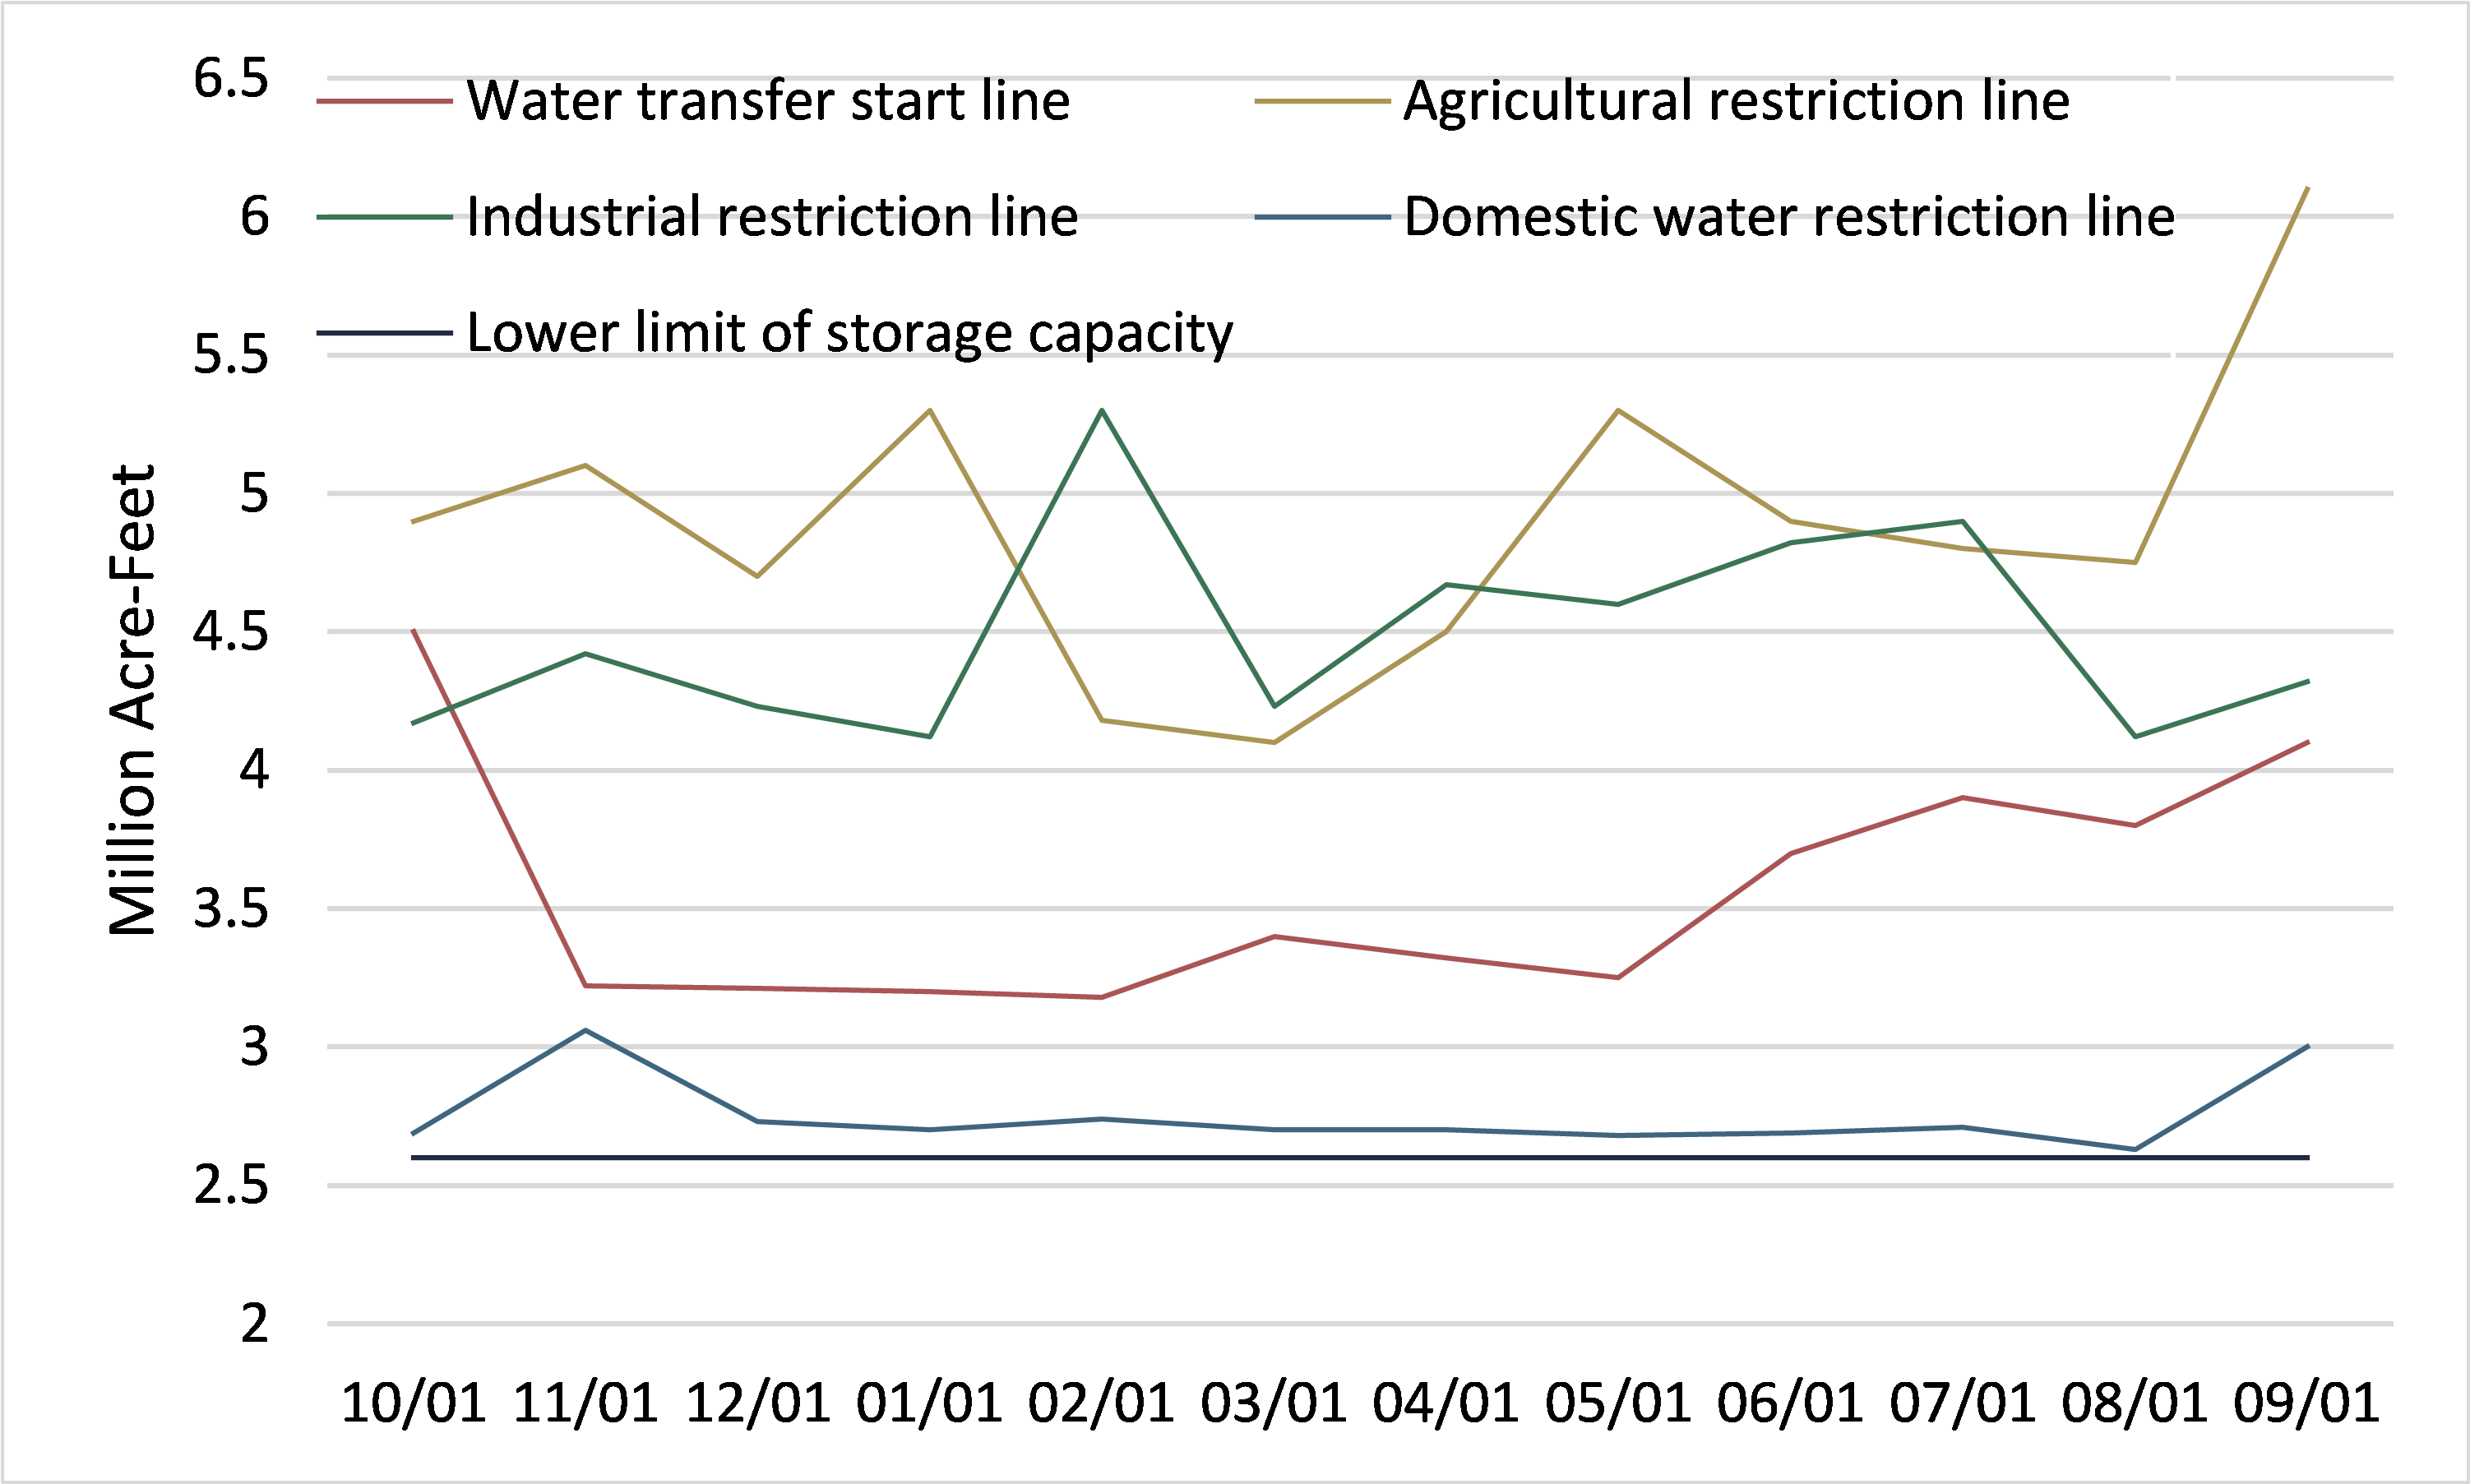
\includegraphics[width=0.8\textwidth]{figures/result.png}
  \label{fig:res2}
  \caption{Water transfer and supply rules of Powell Lake}
\end{figure}
When the storage volume is above the transfer line, no external water transfer will be introduced; on the contrary, external water transfer will be introduced according to the transfer capacity of the period. The higher the transfer line, the higher the chance of transferring water in that month. The start line in the graph indicates that the overall chance of transferring water during the non-flood season is high because the water is less after the end of the flood season.
\par
The reason for this is that urban users have to meet both the high guarantee rate of water supply and the low depth of damage, which requires high water supply, and the chance of water supply being restricted is small. The higher the dispatch line is, the greater the chance that the agricultural customers' water supply will be restricted. This is due to the unevenness of agricultural water demand. Industrial water use is similar.
\par
When water levels in Lake Powell and Lake Mead are high enough, the needs of all users are met; when levels are not high enough, water is allocated according to a reservoir allocation scheme that limits water use.
\par
\begin{figure}[htbp]
  \centering
  \label{fig:hig}
  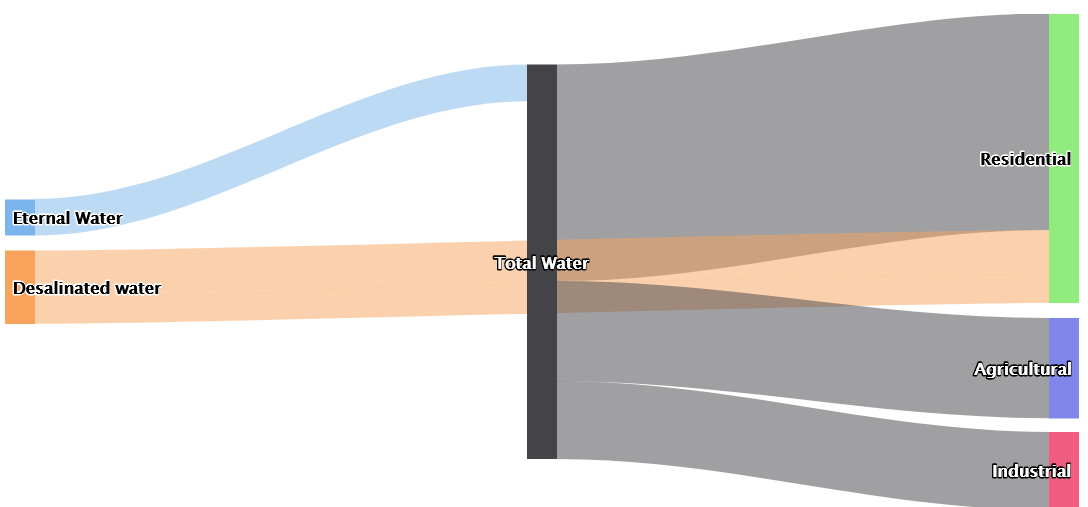
\includegraphics[width=0.6\textwidth]{figures/higchart.png}
  \caption{Water distribution chart for customers with external water sources}
\end{figure}
Figure ~\ref{fig:hig} visualizes the relationship between the allocation of water to users in the presence of external water sources using Sankey diagrams, and the thickness of the line between the water users indicates the magnitude of the water. The higher the allocation of external water sources, the lower the total reservoir water supply, where the external water sources are mainly used for residential and industrial users, and the water that would otherwise be used for these users is allocated to agriculture. This restores water to agriculture, which is squeezed by urban water, while protecting urban water.